\documentclass[12pt]{paper}
\usepackage[english]{babel}
\usepackage{indentfirst}
\usepackage{graphicx}
\usepackage{latexsym}
\usepackage{amsmath}
\usepackage{amsthm}
\usepackage{amssymb,amsfonts}
\usepackage{multicol}
\usepackage{xcolor}
\usepackage{changepage}
\usepackage{hyperref}
\usepackage{fancyhdr}
\usepackage{textcomp}
\usepackage{mathtools}
\usepackage{comment}
\usepackage[normalem]{ulem}
\usepackage{marginnote}
\usepackage[numbers,sort&compress]{natbib}
\mathtoolsset{showonlyrefs=false}

\newcommand{\ga}{\alpha}
\newcommand{\gb}{\beta}
\newcommand{\gam}{\gamma}
\newcommand{\gd}{\delta}
\newcommand{\eps}{\epsilon}
\newcommand{\veps}{\varepsilon}
\newcommand{\gz}{\zeta}
\newcommand{\gt}{\theta}
\newcommand{\gi}{\iota}
\newcommand{\gk}{\kappa}
\newcommand{\gl}{\lambda}
\newcommand{\gs}{\sigma}
\newcommand{\go}{\omega}
\newcommand{\Gam}{\Gamma}
\newcommand{\gD}{\Delta}
\newcommand{\gT}{\Theta}
\newcommand{\gL}{\Lambda}
\newcommand{\gS}{\Sigma}
\newcommand{\gO}{\Omega}

%%%%%%%%%

\newcommand{\pt}[1]{\left( #1\right)}
\newcommand{\pq}[1]{\left[ #1 \right]}
\newcommand{\pg}[1]{\left\{ #1\right\}}
\newcommand{\figref}[1]{\figurename~\ref{#1}}
\newcommand{\red}[1]{\textcolor{red}{#1}}
\newcommand{\blue}[1]{\textcolor{blue}{#1}}
\newcommand{\gray}[1]{\textcolor{gray}{#1}}
\newcommand{\wikilink}[2] { \href{#1.pdf}{#2}\,(\href{#1.tex}{edit})}

\setlength{\textheight}{20cm}
\changepage{2.5cm}{3.0cm}{-4cm}{-1.0cm}{-2cm}{-2cm}{-0.6cm}{0.5cm}{0cm}
\pagestyle{fancy}
\lhead{\bf \today}
\chead{\bf }
\rhead{EG}
\title{O\today}
\author{EG}
\date{\today}

\begin{document}
 \maketitle
\wikilink{home}{Home}

\wikilink{ideas}{Ideas}
 
\section{We use hydrophobic effect to solve Flory problem}

Hydrophobic effect is an effect which lays in the core of protein folding. It is mostly an 
entropic effect originating from the disruption of hydrogen bonds between water 
molecules by the nonpolar solute. \cite{Silverstein1998}. When hydrophobic molecules are placed in 
the water, water molecules form cage-like structures around them (see fig. 
\ref{fig:hydro-effect}). 
When hydrophobes come into contact, water molecules get released; this increases entropy and 
therefore decreases free energy. This decreases in free energy allows proteins keep a tight 
hydrophobic core.
\begin{figure}[h!]
  \centering
  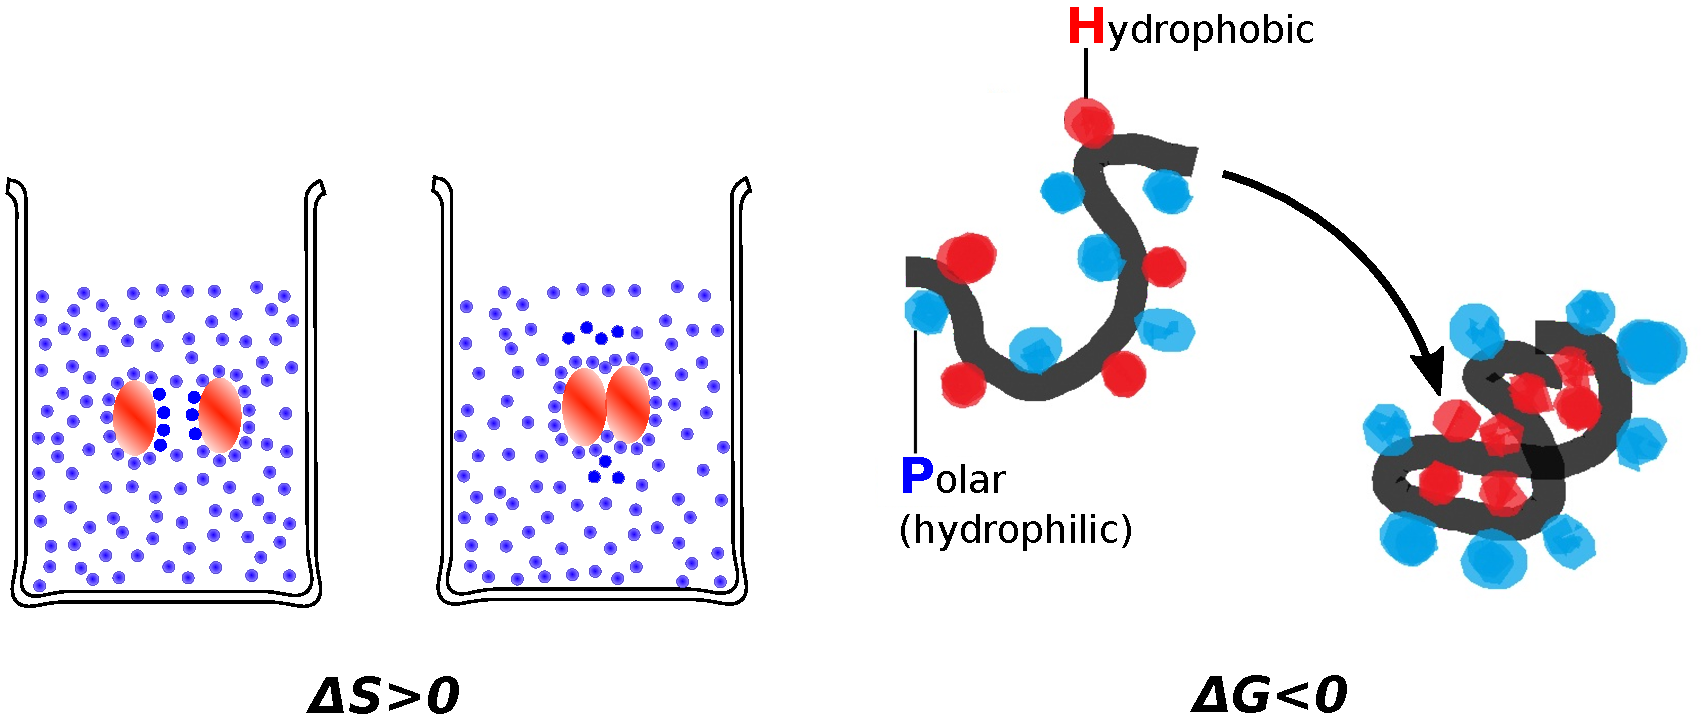
\includegraphics[width=0.7\textwidth]{pictures/hydrophobic-effect.pdf} 
  \caption{Hydrophobic effect is an entropic effect originating from the disruption of 
hydrogen bonds between water molecules by the non-polar solute.
When hydrophobic molecules are placed in the water, water molecules form cage-like 
structures around them. When hydrophobes come into contact, water 
molecules get released; this increases entropy and therefore decreases free energy. }
  \label{fig:hydro-effect}
\end{figure}

\subsection{We use HP model to represent prebiotic polymerization}
To describe effect of hydrophobic interaction on prebiotic polymerization, we adopt the HP model 
-- one of the simplest models of proteins; it's well studied and sequence space is well 
understood\cite{lau1989lattice,Chan1991,Miller1995,Yue1995,agarwala1997local}. While initially HP 
model was introduced as a model for proteins, we are indifferent to exact chemical nature of the 
prebiotic polymers and consider only principles of spontaneous polymerization.
\paragraph{HP model features:} 
\begin{itemize}
 \item It is a two dimensional square lattice model of protein folding
 \item It has 2 types of monomers: hydrophobic (H) and polar (P). 
 \item HP model has a folding code: presence of hydrophobic interaction makes some conformations 
of the same chain more energetically favorable than others. Moreover certain chains will have a 
unique conformation, which delivers free energy minimum. This conformations are called native 
states, and sequences, which have native state, are considered being capable of folding (see fig. 
\ref{fig:hp-model} ).
\end{itemize}

\begin{figure}[h!]
  \centering
  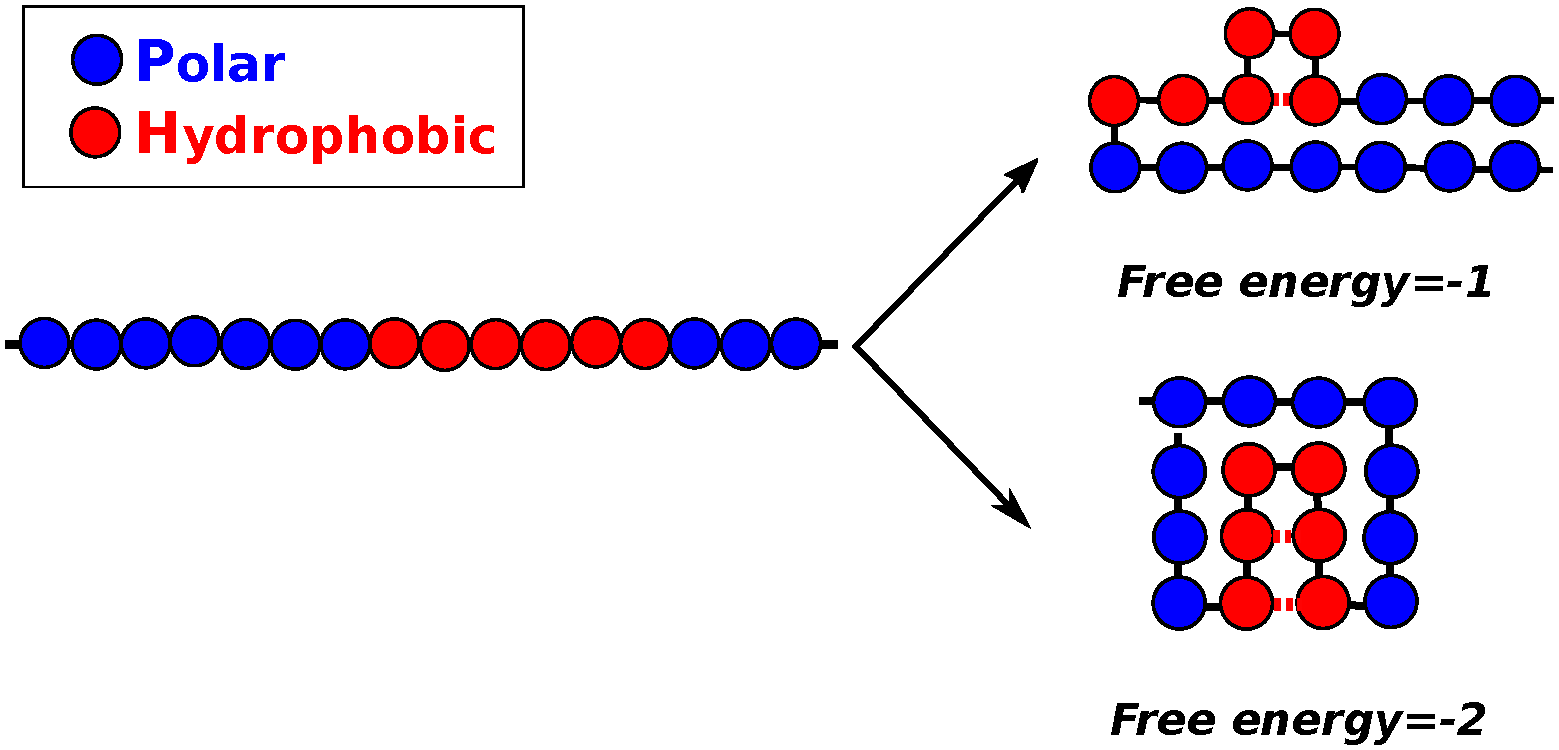
\includegraphics[width=0.6\textwidth]{pictures/hp-model.pdf} 
  \caption{}
  \label{fig:hp-model}
\end{figure}
Because of the ability to form hydrophobic contacts in water, even hetero-polymers that 
are as simple as HP-polymers will often fold up, even as short chains. 
While short HP chains will not necessarily have great stability qualities (they will often be 
fairly amorphous ``oil-drop''-like balls that are ensembles of conformations), some HP 
sequences will fold more uniquely than others. Latter will spend most of the time in the native 
state. And, what is important, it has been shown that a 
relatively large fraction of sequence space will fold to compact structures or compact ensemble 
structures\cite{lau1989lattice}.

\subsection{HP-foldamers can work as prebiotic catalysts}
Our central premise is that the same promiscuous hydrophobic interactions that can cause random 
HP heteropolymers to collapse into compact, folded, structures. However hydrophobic 
interaction will also cause polymer-polymer attraction and binding between molecules.  In some 
cases, a folded HP-polymers can provide a hydrophobic ``landing site'' for another HP polymer 
and/or another H monomer (see fig. \ref{fig:hp-catalysis}).  


When a folded chain has exposed hydrophobic monomers on its surface it can attract another chain 
with hydrophobes as well as activated hydrophobic monomer. Interaction between 3 of them localizes 
growing chain and next monomer (fig.\ref{fig:hp-catalysis}(a)). In addition to that, hydrophobic 
interaction also lowers activation barrier of the polymerization reaction, accelerating reaction 
this way.

One hydrophobic interaction is about $1-2kT$. Given that rate of catalysis is proportional to an 
exponent of the activation barrier, 3-4 hydrophobic interactions are enough to increase 
polymerization rate $\approx 100$ times (fig.\ref{fig:hp-catalysis}(b)). 
Of course, this is not a good rate enhancement, compared to $2\cdot10^7$-fold rate enhancement 
brought about
by modern ribosomes\cite{Sievers2004a}. However the very 
first catalysts don't have to be very efficient: their purpose is to create a driving force of 
evolution.

HP-catalysis drives addition of hydrophobes to hydrophobes. A seemingly logical conclusion would 
be that one will end up with purely hydrophobic polymers. However this is not true. Sequences 
capable of catalysis must have a relatively stable structure. Purely hydrophobic sequences don't 
have this property: they have very many conformational states with the same low free energy. 
Therefore they will spend a lot of time jumping between those states and their bonds will be 
affected by hydrolysis. They also will not be able serve as catalysts. Sequences with $50-80\%$ 
of hydrophobes, on the other hand, will have the most stable structures; they will 
be protected from hydrolysis and will be able to localize growing chain with the next added 
monomer.
\begin{figure}[h!]
  \centering
  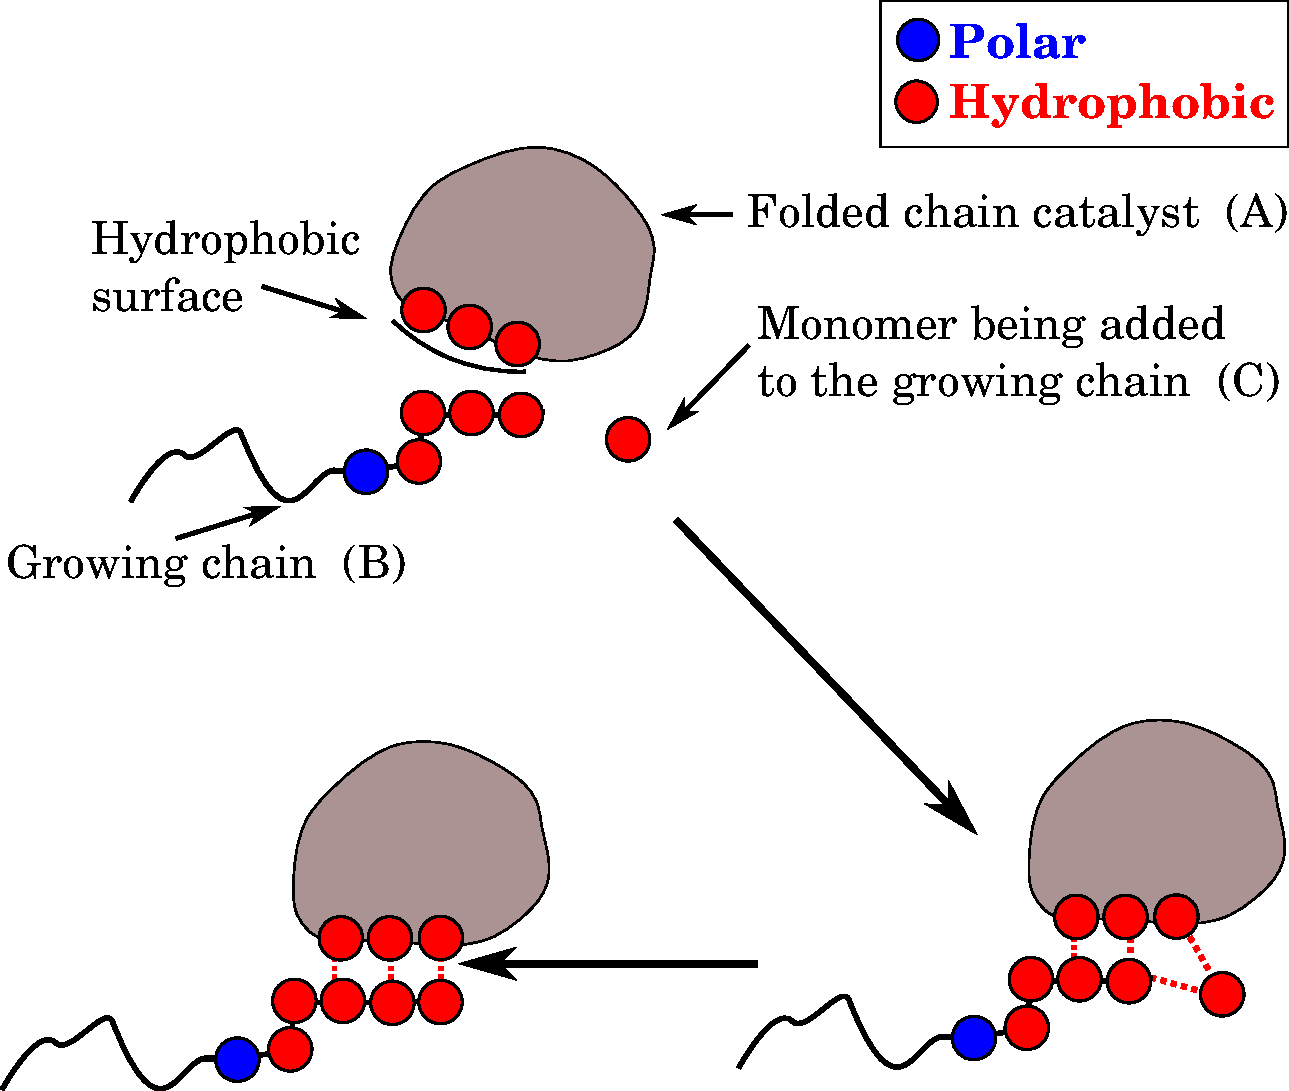
\includegraphics[width=0.85\textwidth]{pictures/hp-catalysis.pdf} 
  \caption{Catalyst catalyzes a growing of an unfolded hp-polymer. 
           Having just 3-4 hydrophobic contacts is enough to lower an 
           activation barrier for $\propto 100$ times at room 
           temperature.}
  \label{fig:hp-catalysis}
\end{figure}



  \bibliography{/data/research/31.mendeleyBibtex/library}
  \bibliographystyle{unsrt}

\end{document}
